\documentclass[letterpaper,10pt]{article}

\usepackage{enumitem}
\usepackage{titling}
\usepackage{listings}
\usepackage{url}
\usepackage{hyperref}
\usepackage{setspace}
\usepackage{subfig}
\usepackage{sectsty}
\usepackage{pdfpages}
\usepackage{colortbl}
\usepackage{multirow}
\usepackage{multicol}
\usepackage{relsize}
\usepackage{amsmath}
\usepackage{wasysym}
\usepackage{fancyvrb}
\usepackage[yyyymmdd]{datetime}
\usepackage{amsmath,amssymb,amsthm,graphicx,xspace}
\usepackage[titlenotnumbered,noend,noline]{algorithm2e}
\usepackage[compact]{titlesec}
\usepackage{XCharter}
\usepackage[T1]{fontenc}
\usepackage[scaled]{beramono}
\usepackage[normalem]{ulem}
\usepackage{booktabs}
\usepackage{tikz}
\usetikzlibrary{arrows,automata,shapes,trees,matrix,chains,scopes,positioning,calc}
\tikzstyle{block} = [rectangle, draw, fill=blue!20,
text width=2.5em, text centered, rounded corners, minimum height=2em]
\tikzstyle{bw} = [rectangle, draw, fill=blue!20,
text width=4em, text centered, rounded corners, minimum height=2em]

\definecolor{namerow}{cmyk}{.40,.40,.40,.40}
\definecolor{namecol}{cmyk}{.40,.40,.40,.40}
\renewcommand{\dateseparator}{-}

\let\LaTeXtitle\title
\renewcommand{\title}[1]{\LaTeXtitle{\textsf{#1}}}

\lstset{basicstyle=\footnotesize\ttfamily,breaklines=true}

\newcommand{\handout}[5]{
	\noindent
	\begin{center}
		\framebox{
			\vbox{
				\hbox to 5.78in { {\bf ECE 252: Systems Programming and Concurrency } \hfill #2 }
				\vspace{4mm}
				\hbox to 5.78in { {\Large \hfill #4  \hfill} }
				\vspace{2mm}
				\hbox to 5.78in { {\em #3 \hfill \today} }
			}
		}
	\end{center}
	\vspace*{4mm}
}

\newcommand{\lecture}[3]{\handout{#1}{#2}{#3}{Lecture#1}}
\newcommand{\tuple}[1]{\ensuremath{\left\langle #1 \right\rangle}\xspace}

\newcommand{\Rplus}{\protect\hspace{-.1em}\protect\raisebox{.35ex}{\smaller{\smaller\textbf{+}}}}
\newcommand{\Cpp}{\mbox{C\Rplus\Rplus}\xspace}


\addtolength{\oddsidemargin}{-1.000in}
\addtolength{\evensidemargin}{-0.500in}
\addtolength{\textwidth}{2.0in}
\addtolength{\topmargin}{-1.000in}
\addtolength{\textheight}{1.75in}
\addtolength{\parskip}{\baselineskip}
\setlength{\parindent}{0in}
\renewcommand{\baselinestretch}{1.5}
\newcommand{\term}{Spring 2019}
\newcommand{\termnumeric}{1195}

\singlespace


\begin{document}

\lecture{ 26 --- The Byzantine Generals Problem }{\term}{Jeff Zarnett}

\section*{Istanbul was Constantinople}
Byzantium was an ancient Greek city, rebuilt by Constantine the Great under the name of Constantinople. It is now modern day Turkey. The word Byzantine refers to things relating to the empire based there, but in English has also come to mean a thing that is excessively complicated. But it's the last ``extra'' meaning that we want to talk about: characterized by deviousness. The Byzantine Empire was characterized by deviousness, alright: it was a place where generals and leaders would vie for power in underhanded ways, backstabbing and sabotaging others when they thought it was to their advantage. I guess it was very \textit{Game of Thrones}, now that I think of it.

Where this crosses over into the realm of programming is in dealing with the unreliable nature of systems. It's not that we think that somewhere out there one of the processes in the system is malicious and trying to make the system fail... although that could happen... but our normal expectation is that the systems interacting may be faulty or have errors or bugs, not malicious intent.

However we get here, though, we still need a way to deal with the fact that not everyone agrees and sometimes messages get mixed up. And that is a communication problem, yes, but also a coordination problem as well. And if you've tried to get a group of five people to agree on where to go to lunch you may have found it unexpectedly difficult... now imagine that one person is (unintentionally or otherwise) trying to sabotage the planning so organizing lunch will fail.

The generic form of the Byzantine Generals problem looks something like this. There is a \textit{General} who is giving the orders. There are also $n$ \textit{Lieutenants} who each are commanding a group of the Empire's troops. The individual troops just do what they're told so there's no further concern for their actions. The lieutenants can communicate with one another through messages, and they get their orders from the general. All of the lieutenants have to work together for their plan to be a success, otherwise there is chaos.

No problem, you might imagine. The general tells the lieutenants what to do and they do it! And if one of the lieutenants does the wrong thing, that lieutenant is a traitor. But it's not so simple, because the general can be disloyal too. Horrible Bosses: Byzantium!

Suppose you are a disloyal general. Your Emperor has commanded you to attack, but you want the attack to fail, but also seem like it's not your fault. What do you do? You can issue different orders to different lieutenants, they will be all confused and uncoordinated, and oh gee darn, I guess the attack didn't go as planned! And you can blame the lieutenants who are now dead for going too early, or something, because it's not like they can defend themselves now...

So a loyal general sends the same message to all lieutenants and a disloyal one sends different messages to different lieutenants. It's key to remember that ``loyal'' really means ``functioning'' and ``disloyal'' means ``faulty''~\cite{mte241}. It's fun to make it seem like human actors are doing things for their own evil-villainy-related reasons, but it is just computer interaction that presumably has no actual malicious intent. It's also worth noting that being in one state or the other is not permanent: a functioning unit can be damaged, a malfunctioning one can be repaired, or a problem can be transient (i.e., some electromagnetic interference flipped a bit here or there) and resolve itself with no further action.

One of the key decisions is about how much disloyalty your system can tolerate. Given enough bad actors, things will go wrong. If everyone is disloyal, utter chaos will result. But is it enough to tolerate one disloyal participant? Two? The line will have to be drawn somewhere... But at the very least we don't want to let one disloyal individual ruin things for everyone, even if that disloyal individual is the boss.

\subsection*{Should I Stay or Should I Go Now?}
In the examples that we will discuss there are two kinds of command: attack and retreat. In a real system the options don't have to be quite so binary (we could give any orders) but for the purpose of demonstration and coming to grips with this problem we'll use the binary example. Attack or retreat.

It is possible that our system produces a tie (no matter how many participants or possible actions we have). This usually necessitates a default action be selected. So if we cannot come to a decision, we take the default choice. Usually we say that the default choice is to retreat.

Consider the  diagram below where we have a disloyal general, and two loyal lieutenants. In our examples in this section we'll use G for generals, L for lieutenants, and we'll make disloyal participants red and loyal ones grey.

\begin{center}
	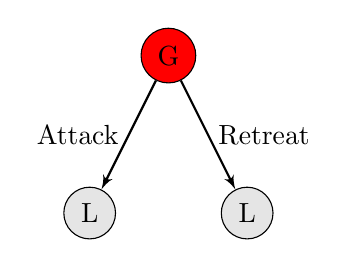
\begin{tikzpicture}
		\node[circle,draw,fill=red, minimum size=0.5] (G) at (0, 0) {G};
		\node[circle,draw,fill=gray!20, minimum size=0.5] (L1) at (-1, -2) {L};
		\node[circle,draw,fill=gray!20, minimum size=0.5] (L2) at (1, -2) {L};
		\draw[-latex', thick] (G) -- (L1) node[midway, left]{Attack};
		\draw[-latex', thick] (G) -- (L2) node[midway, right]{Retreat};
	\end{tikzpicture}
\end{center}

What are lieutenants to do? In the imperfect world of Byzantium the lieutenants can try to figure out if they're about to be mismanaged to literal death by communicating with one another. If they are all on the same page then they can do what they're supposed to do; if they're not, then they will fall back on the default option.

Unfortunately, though, letting the lieutenants communicate is not a complete solution. Because lieutenants can lie, even if the general doesn't.

\begin{center}
	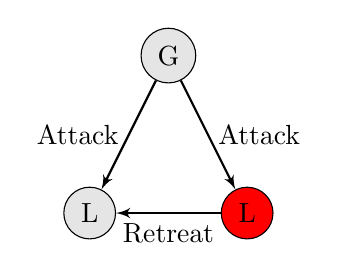
\begin{tikzpicture}
		\node[circle,draw,fill=gray!20, minimum size=0.5] (G) at (0, 0) {G};
		\node[circle,draw,fill=gray!20, minimum size=0.5] (L1) at (-1, -2) {L};
		\node[circle,draw,fill=red, minimum size=0.5] (L2) at (1, -2) {L};
		\draw[-latex', thick] (G) -- (L1) node[midway, left]{Attack};
		\draw[-latex', thick] (G) -- (L2) node[midway, right]{Attack};
		\draw[-latex', thick] (L2) -- (L1) node[midway, below]{Retreat};
	\end{tikzpicture}
\end{center}

In general if there are $d$ disloyal participants, we will need there to be more than $3d$ participants for the loyal lieutenants to agree on what to do. If the general is loyal, then at least $2d$ loyal lieutenants are needed to obey the orders; if the general is disloyal then $2d+1$ loyal lieutenants are needed so they can come up with a course of action~\cite{mte241}.

Let's imagine that there is at most one disloyal participant. If that's the case then all lieutenants should compare notes and decide on the majority course of action. Each lieutenant compiles a little table (or array or vector, whatever) of the data received and then decide on what the majority cause of action is. It might be simpler to just count the total number of votes, but it would make it harder to figure out later who the traitor is (if there is one).

What if we can have two disloyal participants? Each lieutenant sending its messages and using a majority-wins vote isn't necessarily going to work here. It can happen that the general is disloyal and one of the lieutenants is a collaborator. Consider this scenario below from~\cite{mte241} where the general is disloyal and sends mixed instructions. What can the collaborating lieutenant do to make sure that the other lieutenants don't come to an agreement?

\begin{center}
	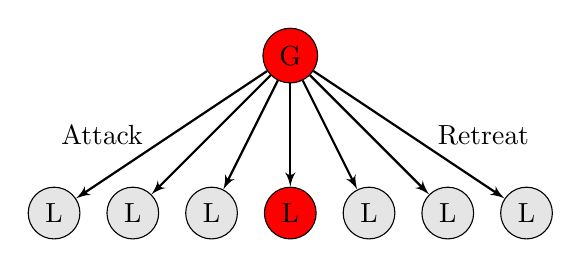
\begin{tikzpicture}
		\node[circle,draw,fill=red, minimum size=0.5] (G) at (0, 0) {G};
		\node[circle,draw,fill=gray!20, minimum size=0.5] (L1) at (-3, -2) {L};
		\node[circle,draw,fill=gray!20, minimum size=0.5] (L2) at (-2, -2) {L};
		\node[circle,draw,fill=gray!20, minimum size=0.5] (L3) at (-1, -2) {L};
		\node[circle,draw,fill=red, minimum size=0.5] (L4) at (0, -2) {L};
		\node[circle,draw,fill=gray!20, minimum size=0.5] (L5) at (1, -2) {L};
		\node[circle,draw,fill=gray!20, minimum size=0.5] (L6) at (2, -2) {L};
		\node[circle,draw,fill=gray!20, minimum size=0.5] (L7) at (3, -2) {L};

		\draw[-latex', thick] (G) -- (L1) node[midway, left]{Attack~~~};
		\draw[-latex', thick] (G) -- (L2);
		\draw[-latex', thick] (G) -- (L3);
		\draw[-latex', thick] (G) -- (L4);
		\draw[-latex', thick] (G) -- (L5);
		\draw[-latex', thick] (G) -- (L6);
		\draw[-latex', thick] (G) -- (L7) node[midway, right]{~~Retreat};
	\end{tikzpicture}
\end{center}

The lieutenants all send one another their instructions. Each of the loyal lieutenants sends its received command and received the honest answer from three other lieutenants. The score is 3 attack and 3 retreat. The disloyal lieutenant sends one message to half the other participants, and a different message to the other half.

\begin{center}
	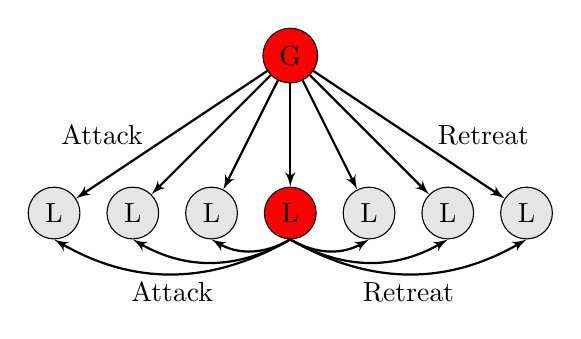
\begin{tikzpicture}
		\node[circle,draw,fill=red, minimum size=0.5] (G) at (0, 0) {G};
		\node[circle,draw,fill=gray!20, minimum size=0.5] (L1) at (-3, -2) {L};
		\node[circle,draw,fill=gray!20, minimum size=0.5] (L2) at (-2, -2) {L};
		\node[circle,draw,fill=gray!20, minimum size=0.5] (L3) at (-1, -2) {L};
		\node[circle,draw,fill=red, minimum size=0.5] (L4) at (0, -2) {L};
		\node[circle,draw,fill=gray!20, minimum size=0.5] (L5) at (1, -2) {L};
		\node[circle,draw,fill=gray!20, minimum size=0.5] (L6) at (2, -2) {L};
		\node[circle,draw,fill=gray!20, minimum size=0.5] (L7) at (3, -2) {L};

		\draw[-latex', thick] (G) -- (L1) node[midway, left]{Attack~~~};
		\draw[-latex', thick] (G) -- (L2);
		\draw[-latex', thick] (G) -- (L3);
		\draw[-latex', thick] (G) -- (L4);
		\draw[-latex', thick] (G) -- (L5);
		\draw[-latex', thick] (G) -- (L6);
		\draw[-latex', thick] (G) -- (L7) node[midway, right]{~~Retreat};
		\draw[-latex', thick] (L4.south) to [bend right] (L7.south);
		\draw[-latex', thick] (L4.south) to [bend right] (L6.south);
		\draw[-latex', thick] (L4.south) to [bend right] (L5.south);
		\draw[-latex', thick] (L4.south) to [bend left] (L3.south);
		\draw[-latex', thick] (L4.south) to [bend left] (L2.south);
		\draw[-latex', thick] (L4.south) to [bend left] (L1.south);

		\node at(-1.5, -3) {Attack};
		\node at(1.5, -3) {Retreat};
	\end{tikzpicture}
\end{center}

Now we're in trouble because half the participants think the majority action is attack and half the participants think the majority action is retreat. Summing up what we heard is not sufficient. Lieutenants should also talk about what they heard from one another. After the general issues instructions, each lieutenant should then communicate with every other to hear what the general said to them. Then by reviewing this information, they can decide what to do.

Consider a simple example where the general is loyal and we have two traitorous lieutenants with a total of seven participants. The general issued an order to attack.

\begin{center}
	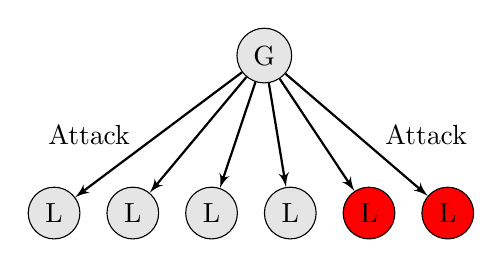
\begin{tikzpicture}
		\node[circle,draw,fill=gray!20, minimum size=0.5] (G) at (-0.33, 0) {G};
		\node[circle,draw,fill=gray!20, minimum size=0.5] (L1) at (-3, -2) {L};
		\node[circle,draw,fill=gray!20, minimum size=0.5] (L2) at (-2, -2) {L};
		\node[circle,draw,fill=gray!20, minimum size=0.5] (L3) at (-1, -2) {L};
		\node[circle,draw,fill=gray!20, minimum size=0.5] (L4) at (0, -2) {L};
		\node[circle,draw,fill=red, minimum size=0.5] (L5) at (1, -2) {L};
		\node[circle,draw,fill=red, minimum size=0.5] (L6) at (2, -2) {L};

		\draw[-latex', thick] (G) -- (L1) node[midway, left]{Attack~~~};
		\draw[-latex', thick] (G) -- (L2);
		\draw[-latex', thick] (G) -- (L3);
		\draw[-latex', thick] (G) -- (L4);
		\draw[-latex', thick] (G) -- (L5);
		\draw[-latex', thick] (G) -- (L6) node[midway, right]{~~Attack};
	\end{tikzpicture}
\end{center}


So each lieutenant constructs the following vector. We're not sure if the general is a traitor, but we'll take notes from every other participant, and see what they report. The general form is as follows, where $v_{x}$ is the forwarded order we received from lieutenant $x$:

\begin{center}
	\begin{tabular}{|l|l|l|l|l|l|l|l|}
		\hline
		General & L1      & L2      & L3      & L4      & L5      & L6      \\
		\hline
		?       & $v_{1}$ & $v_{2}$ & $v_{3}$ & $v_{4}$ & $v_{5}$ & $v_{6}$ \\
		\hline
	\end{tabular}
\end{center}

So if we are lieutenant 1, we complete the table as below. The value for L1 is what we received from the general, but we get the remaining values from the other lieutenants.

\begin{center}
	\begin{tabular}{|l|l|l|l|l|l|l|l|}
		\hline
		General & L1 & L2 & L3 & L4 & L5 & L6 \\
		\hline
		?       & A  & A  & A  & A  & R  & R  \\
		\hline
	\end{tabular}
\end{center}


Then the lieutenants just compare notes on this subject as well! They send to one another their vectors and assemble them into a table. Whatever lieutenant $x$ received in the first round forms row $x$ of the table, and the other rows are added from this second round of communication. In the table each value $v_{i,j}$ is interpreted as ``Lieutenant $i$ says that Lieutenant $j$ reports the general said $v$''. The entries on the diagonal are redundant because of course each lieutenant agrees with itself:

\begin{center}
	\begin{tabular}{|l|l|l|l|l|l|l|l|}
		\hline
		General & L1        & L2        & L3        & L4        & L5        & L6        \\
		\hline
		?       & $v_{1,1}$ & $v_{1,2}$ & $v_{1,3}$ & $v_{1,4}$ & $v_{1,5}$ & $v_{1,6}$ \\\hline
		?       & $v_{2,1}$ & $v_{2,2}$ & $v_{2,3}$ & $v_{2,4}$ & $v_{2,5}$ & $v_{2,6}$ \\\hline
		?       & $v_{3,1}$ & $v_{3,2}$ & $v_{3,3}$ & $v_{3,4}$ & $v_{3,5}$ & $v_{3,6}$ \\\hline
		?       & $v_{4,1}$ & $v_{4,2}$ & $v_{4,3}$ & $v_{4,4}$ & $v_{4,5}$ & $v_{4,6}$ \\\hline
		?       & $v_{5,1}$ & $v_{5,2}$ & $v_{5,3}$ & $v_{5,4}$ & $v_{5,5}$ & $v_{5,6}$ \\\hline
		?       & $v_{6,1}$ & $v_{6,2}$ & $v_{6,3}$ & $v_{6,4}$ & $v_{6,5}$ & $v_{6,6}$ \\\hline
	\end{tabular}
\end{center}

Those ``redundant'' entries (the ones on the diagonal) need to be removed from the table. From the point of view of lieutenant 1, let's imagine the table looks like this (filling in for the sake of the example that L5 and L6 always say retreat).
\begin{center}
	\begin{tabular}{|l|l|l|l|l|l|l|l|}
		\hline
		General & L1 & L2 & L3 & L4 & L5 & L6 \\
		\hline
		?       & ~  & A  & A  & A  & R  & R  \\ \hline
		?       & A  & ~  & A  & A  & R  & R  \\ \hline
		?       & A  & A  & ~  & A  & R  & R  \\ \hline
		?       & A  & A  & A  & ~  & R  & R  \\ \hline
		?       & R  & R  & R  & R  & ~  & R  \\ \hline
		?       & R  & R  & R  & R  & R  & ~  \\ \hline
	\end{tabular}
\end{center}

One the thing we can do, however, is fill in the first column: lieutenant 1 does not care what other people THINK they said; so the whole column can be replaced with what was actually said:

\begin{center}
	\begin{tabular}{|l|l|l|l|l|l|l|l|}
		\hline
		General & L1 & L2 & L3 & L4 & L5 & L6 \\
		\hline
		?       & ~  & A  & A  & A  & R  & R  \\ \hline
		?       & A  & ~  & A  & A  & R  & R  \\ \hline
		?       & A  & A  & ~  & A  & R  & R  \\ \hline
		?       & A  & A  & A  & ~  & R  & R  \\ \hline
		?       & A  & R  & R  & R  & ~  & R  \\ \hline
		?       & A  & R  & R  & R  & R  & ~  \\ \hline
	\end{tabular}
\end{center}

Then we'll try to figure out the majority vote for each $j$ in the table. So sum up each column:

\begin{center}
	\begin{tabular}{|l|l|l|l|l|l|l|l|}
		\hline
		General & L1 & L2 & L3 & L4 & L5 & L6 \\
		\hline
		?       & A  & A  & A  & A  & R  & R  \\
		\hline
	\end{tabular}
\end{center}

And we have four lieutenants who think the general said attack and two who think the general said retreat. The majority wins and the attack proceeds. Onward to victory, brothers and sisters!

If there was one less loyal lieutenant, though, we could have a tie here which would result in picking the default value. If the general ordered something other than the default value (e.g., default is retreat and the order was attack) the general will not be happy about this...

You may have figured out that since disloyal participants can lie at any step of the equation, we can't rely on their data at all. That's true! In the examples in the course we know that two participants are traitors and I've said they are L5 and L6. Therefore we could replace whatever they say with a question mark in the able rather than any particular answer, because they are liars. In real life though, \textit{some} message is received -- attack or retreat -- and it's only later we could identify which participants are the traitors.

Let's go back to the example of having eight participants: one general and seven lieutenants. So if we are lieutenant 1, we complete the table as below. The value for L1 is what we received from the general, but we get the remaining values from the other lieutenants.

\begin{center}
	\begin{tabular}{|l|l|l|l|l|l|l|l|}
		\hline
		General & L1 & L2 & L3 & L4 & L5 & L6 & L7 \\
		\hline
		?       & A  & A  & A  & A  & R  & R  & R  \\
		\hline
	\end{tabular}
\end{center}

However, if we are lieutenant 7 our vector looks like this instead:

\begin{center}
	\begin{tabular}{|l|l|l|l|l|l|l|l|}
		\hline
		General & L1 & L2 & L3 & L4 & L5 & L6 & L7 \\
		\hline
		?       & A  & A  & A  & R  & R  & R  & R  \\
		\hline
	\end{tabular}
\end{center}

From the point of view of lieutenant 1 the table is formed then as follows:

\begin{center}
	\begin{tabular}{|l|l|l|l|l|l|l|l|}
		\hline
		General & L1 & L2 & L3 & L4 & L5 & L6 & L7 \\
		\hline
		?       & ~  & A  & A  & A  & R  & R  & R  \\ \hline
		?       & A  & ~  & A  & A  & R  & R  & R  \\ \hline
		?       & A  & A  & ~  & A  & R  & R  & R  \\ \hline
		?       & ?  & ?  & ?  & ~  & ?  & ?  & ?  \\ \hline
		?       & A  & A  & A  & R  & ~  & R  & R  \\ \hline
		?       & A  & A  & A  & R  & R  & ~  & R  \\ \hline
		?       & A  & A  & A  & R  & R  & R  & ~  \\ \hline
	\end{tabular}
\end{center}

The fourth row is shown as all question marks. Why? Lieutenant 4 is the traitor and could also lie about what the other lieutenants said. Then replace the first column.

\begin{center}
	\begin{tabular}{|l|l|l|l|l|l|l|l|}
		\hline
		General & L1 & L2 & L3 & L4 & L5 & L6 & L7 \\
		\hline
		?       & ~  & A  & A  & A  & R  & R  & R  \\ \hline
		?       & A  & ~  & A  & A  & R  & R  & R  \\ \hline
		?       & A  & A  & ~  & A  & R  & R  & R  \\ \hline
		?       & A  & ?  & ?  & ~  & ?  & ?  & ?  \\ \hline
		?       & A  & A  & A  & R  & ~  & R  & R  \\ \hline
		?       & A  & A  & A  & R  & R  & ~  & R  \\ \hline
		?       & A  & A  & A  & R  & R  & R  & ~  \\ \hline
	\end{tabular}
\end{center}

Sum up each column:

\begin{center}
	\begin{tabular}{|l|l|l|l|l|l|l|l|}
		\hline
		General & L1 & L2 & L3 & L4 & L5 & L6 & L7 \\
		\hline
		?       & A  & A  & A  & ?  & R  & R  & R  \\
		\hline
	\end{tabular}
\end{center}

Each of the lieutenants figures out that we have a draw and we then choose the default choice. Well, that's grim, but it makes sense: the general issued contradictory orders and the collaborating lieutenant did the same. But now instead of half the lieutenants charging in and dying while the others hang back and watch, everyone takes the same action, even if it's not the one that helps the Empire the most.

If there three disloyal participants can exist in the system there's another round of data exchange that needs to take place. Each lieutenant sends the table formed in the second round to all other lieutenants. The more disloyalty there could be in the system, the more rounds the process will go on. As you may have identified, for $n$ participants the communication grows at $n^{2}$ (well, actually worst case $dn^{2}$~\cite{mte241}) and even worse than that, as the number of participants and rounds increases, the amount of data to be sent also increases. For this reason it is somewhat impractical to tolerate a large number of disloyal participants.

That is, however, still a design decision...

Part of the difficulty comes from the fact that lieutenants can lie about what the general said.  In the time of Byzantium, wax seals were used (hot wax is poured and then a stamp or ring was used to make an imprint on it). In modern times messages can be signed using public-key cryptography. Then participants can check whether the received message was genuine. An order that does not appear genuine can be disregarded, reducing the ability of disloyal lieutenants to cause confusion.

The Byzantine Generals Problem has applicability in all kinds of systems, from space flight to cryptocurrency. Whenever we have multiple ``agents'' of some sort that come to their own conclusions about what to do, we can face this issue. As long as we know this, we can design our system with this in mind, because pretending it's not going to happen is not a real solution...

\bibliographystyle{alphaurl}
\bibliography{252}


\end{document}